% Created 2021-01-11 lun. 17:57
% Intended LaTeX compiler: pdflatex
\documentclass[presentation]{beamer}
\usepackage[utf8]{inputenc}
\usepackage[T1]{fontenc}
\usepackage{graphicx}
\usepackage{grffile}
\usepackage{longtable}
\usepackage{wrapfig}
\usepackage{rotating}
\usepackage[normalem]{ulem}
\usepackage{amsmath}
\usepackage{textcomp}
\usepackage{amssymb}
\usepackage{capt-of}
\usepackage{hyperref}
\usepackage{color}
\usetheme{CambridgeUS}
\setbeamertemplate{navigation symbols}{} % pas de barre de navigation
\usepackage[english]{babel}
\usepackage{lmodern}
\usepackage[matha,mathb]{mathabx}
\usepackage{subfig}
\usepackage{mdframed}
\usepackage{minted}
\usemintedstyle{friendly} % set style if needed, see https://frama.link/jfRr8Lpj
\mdfdefinestyle{mystyle}{linecolor=gray!30,backgroundcolor=gray!30}
\BeforeBeginEnvironment{minted}{%
\begin{mdframed}[style=mystyle]}
\AfterEndEnvironment{minted}{%
\end{mdframed} \medskip}
\usepackage{float}
\usepackage{url}
%% Formatting of verbatim outputs (i.e., outputs of R results):
\DefineVerbatimEnvironment{verbatim}{Verbatim}{%
fontsize = \small,
frame = leftline,
formatcom = {\color{gray!97}}
}
\setbeamertemplate{caption}[numbered]
%% Perso colors
\definecolor{PalePurple}{RGB}{127, 90, 182}
\definecolor{DarkPurple}{RGB}{98, 36, 134}
\definecolor{grey}{RGB}{51, 63, 72}
\setbeamercolor{title}{fg=white, bg=DarkPurple}
\setbeamercolor{frametitle}{fg=black}
\setbeamercolor{structure}{fg=PalePurple}
\setbeamercolor{section in head/foot}{fg=white, bg=PalePurple}
\setbeamercolor{subsection in head/foot}{fg=DarkPurple}
\setbeamercolor{title in head/foot}{fg=white, bg=DarkPurple}
\setbeamercolor{date in head/foot}{fg=grey}
%% Structure of a slide :
\setbeamertemplate{footline}
{
\leavevmode%
\hbox{%
\begin{beamercolorbox}[wd=.75\paperwidth,ht=2.25ex,dp=1ex,center]{title in head/foot}%
\usebeamerfont{author in head/foot}\inserttitle
\end{beamercolorbox}%
%\begin{beamercolorbox}[wd=.3\paperwidth,ht=2.25ex,dp=1ex,center]{section in head/foot}%
%\usebeamerfont{title in head/foot}\insertsection
%\end{beamercolorbox}%
\begin{beamercolorbox}[wd=.25\paperwidth,ht=2.25ex,dp=1ex,center]{date in head/foot}%
\insertframenumber{} / \inserttotalframenumber\hspace*{1ex}
\end{beamercolorbox}}%
\vskip0pt%
}
\usetheme{default}
\author{Frédéric Santos\thanks{frederic.santos@u-bordeaux.fr}}
\date{\today}
\title{Customizing and extending Emacs Speaks Statistics}
\hypersetup{
 pdfauthor={Frédéric Santos},
 pdftitle={Customizing and extending Emacs Speaks Statistics},
 pdfkeywords={},
 pdfsubject={},
 pdfcreator={Emacs 27.1 (Org mode 9.4.4)}, 
 pdflang={English}}
\begin{document}

\maketitle

\section{Introductory words}
\label{sec:org19b3713}
\subsection{Filling your Emacs init file}
\label{sec:orgd7c8dcc}
\begin{frame}[label={sec:orgf1d6ad4},fragile]{A word about \texttt{use-package}}
 In this document, several pieces of Emacs Lisp code will be proposed so that you can use them in your init file.

It is assumed that you use \href{https://jwiegley.github.io/use-package/}{\texttt{use-package}} for your init file: the Emacs Lisp code can be adapted in a straightforward manner if you do not use it.

As a reminder, this is the minimal code to add in your init file so as to use \texttt{use-package}, once it has been installed:

\begin{minted}[]{common-lisp}
(unless (package-installed-p 'use-package)
  (package-refresh-contents)
  (package-install 'use-package))
(eval-when-compile
  (require 'use-package))
\end{minted}
\end{frame}

\section{ESS customization}
\label{sec:org1981b77}
\subsection{Visibility of evaluation}
\label{sec:orgd32abb0}
\subsection{Window management}
\label{sec:org22800c1}
\subsection{Syntax highlighting}
\label{sec:orgf5a5bd3}
\subsection{Syntax checker}
\label{sec:orgb6db3bc}
\subsection{Rdired buffers}
\label{sec:org98846b0}

\section{Some useful Emacs packages}
\label{sec:org476d1c8}
\subsection{company}
\label{sec:orgf8f9863}
\subsection{company-quickhelp}
\label{sec:org1d87260}
\begin{frame}[fragile,allowframebreaks,label=]{Documentation popups}
 \href{https://github.com/company-mode/company-quickhelp}{\texttt{company-quickhelp}} allows for documentation popups, e.g. to further describe function arguments.

\begin{figure}[htbp]
\centering
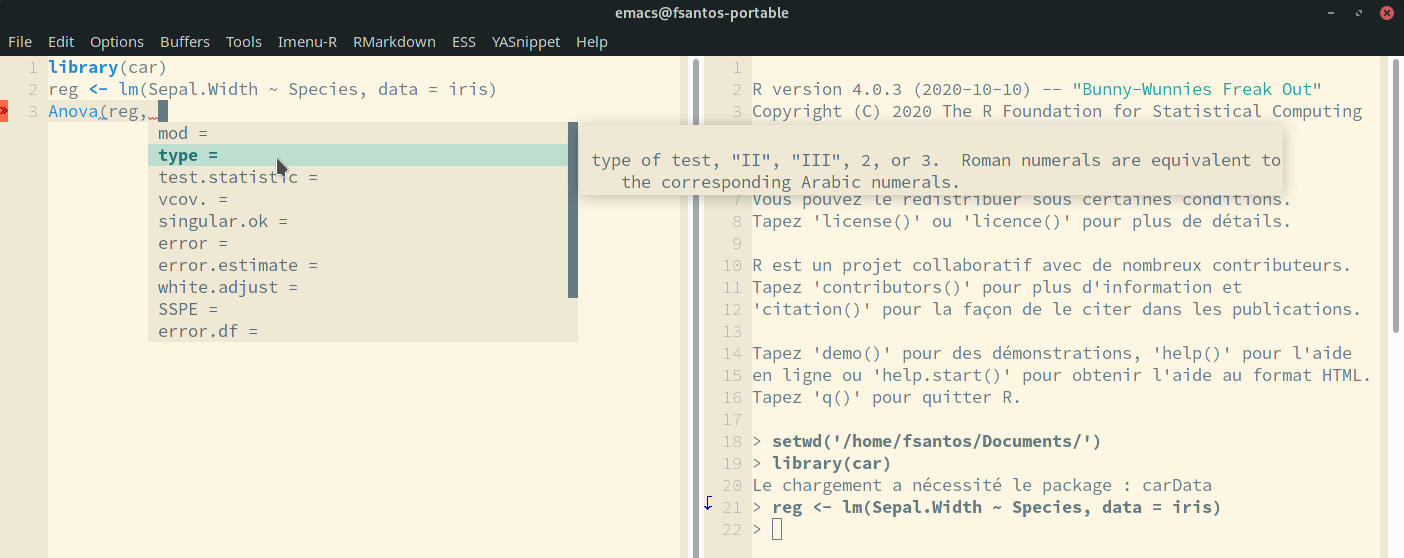
\includegraphics[width=\textwidth]{./images/company-quickhelp.png}
\caption{Documentation popups with \texttt{company-quickhelp}.}
\end{figure}

The minimal elisp code to add to your init file is straightforward:

\begin{minted}[]{common-lisp}
(use-package company-quickhelp
  :ensure t
  :config
  ;; Load company-quickhelp globally:
  (company-quickhelp-mode)
  ;; Time before display of documentation popup:
  (setq company-quickhelp-delay 0.3))
\end{minted}

By default, the documentation popup is shown automatically. You can adjust the time before the popup shows up by customizing the variable \texttt{company-quickhelp-delay}.
\end{frame}

\subsection{yasnippet}
\label{sec:org5c3f02e}
\end{document}